\subsection{Verstellmechanik}
\label{verstellmechanik}
\textit{(ygu)} Die Hauptaufgabe der Verstellmechanik ist die automatisierte Einstellung aller geforderten Topfradien. Die Verstellmechanik bildet einen Teil der Setzeinheit. Dabei kann keine klare Abgrenzung zur Setzeinheit gemacht werden, da in gewissen Komponenten Funktionen beider Einheiten vereint sind. Auch ist die Verstellmechanik klar als Wunschanforderung formuliert. Die Wunschanforderung birgt einen erhöhten Entwicklungsaufwand. Dieser Mehraufwand wird bewusst eingegangen, um ein Maximum an Automatisierungsgrad zu erreichen. Sollte trotzdem auf die automatische Verstellung der Topfradien verzichtet werden, ist die Entwicklung der Pflichtanforderung weniger zeitintensiv und rasch implementiert.
\newline
\subsubsection{Aufbau}
Die Konstruktion der Verstellmechanik basiert auf dem erstellten Funktionsmuster. Die Grundidee ist, dass über zwei Kulissen (eine radiale und eine lineare) der Topfradius zentral an einer Welle verstellt werden kann. Ein klarer Vorteil ist, dass dadurch nur ein Aktor für die Verstellung aller Stechdorne benötigt wird. Die Konstruktion kann in zwei Teile unterteilt werden:
\begin{itemize}
	\item \textbf{dynamischer Teil}: Dieser Teil wird durch die Spindel bewegt. Die drei Stechdorne (Punkt 4 in Abb. \ref{fig:details_vm}) sind durch zwei Kulissen (2, 3) verstellbar gelagert. Durch die Verbindung Keilnabe (5) - Keilwelle (1) sind diese mit dem statischen Teil gekoppelt. Eine geringes Gewicht des bewegten Teils ist für die Beschleunigung dieser Masse essentiell.
	
	\item \textbf{statischer Teil:} Der statische Teil dieser Einheit führt die Verstellung der Topfradien aus. Ein Getriebemotor (8), welcher durch eine Kupplung (9) mit der Keilwelle verbunden ist, führt die Verstellung der Topfradien aus. Diese Umsetzung besticht dadurch, dass anhand der Verbindung Keilnabe (5) - Keilwelle (1) bedeutend weniger Masse translatorisch beschleunigt wird. Dies bringt wertvolle Gewichteinsparnisse und wirkt sich positiv auf das benötigte Beschleunigungsdrehmoment M\textsubscript{a} aus.
\end{itemize}
	\begin{figure}[H]
	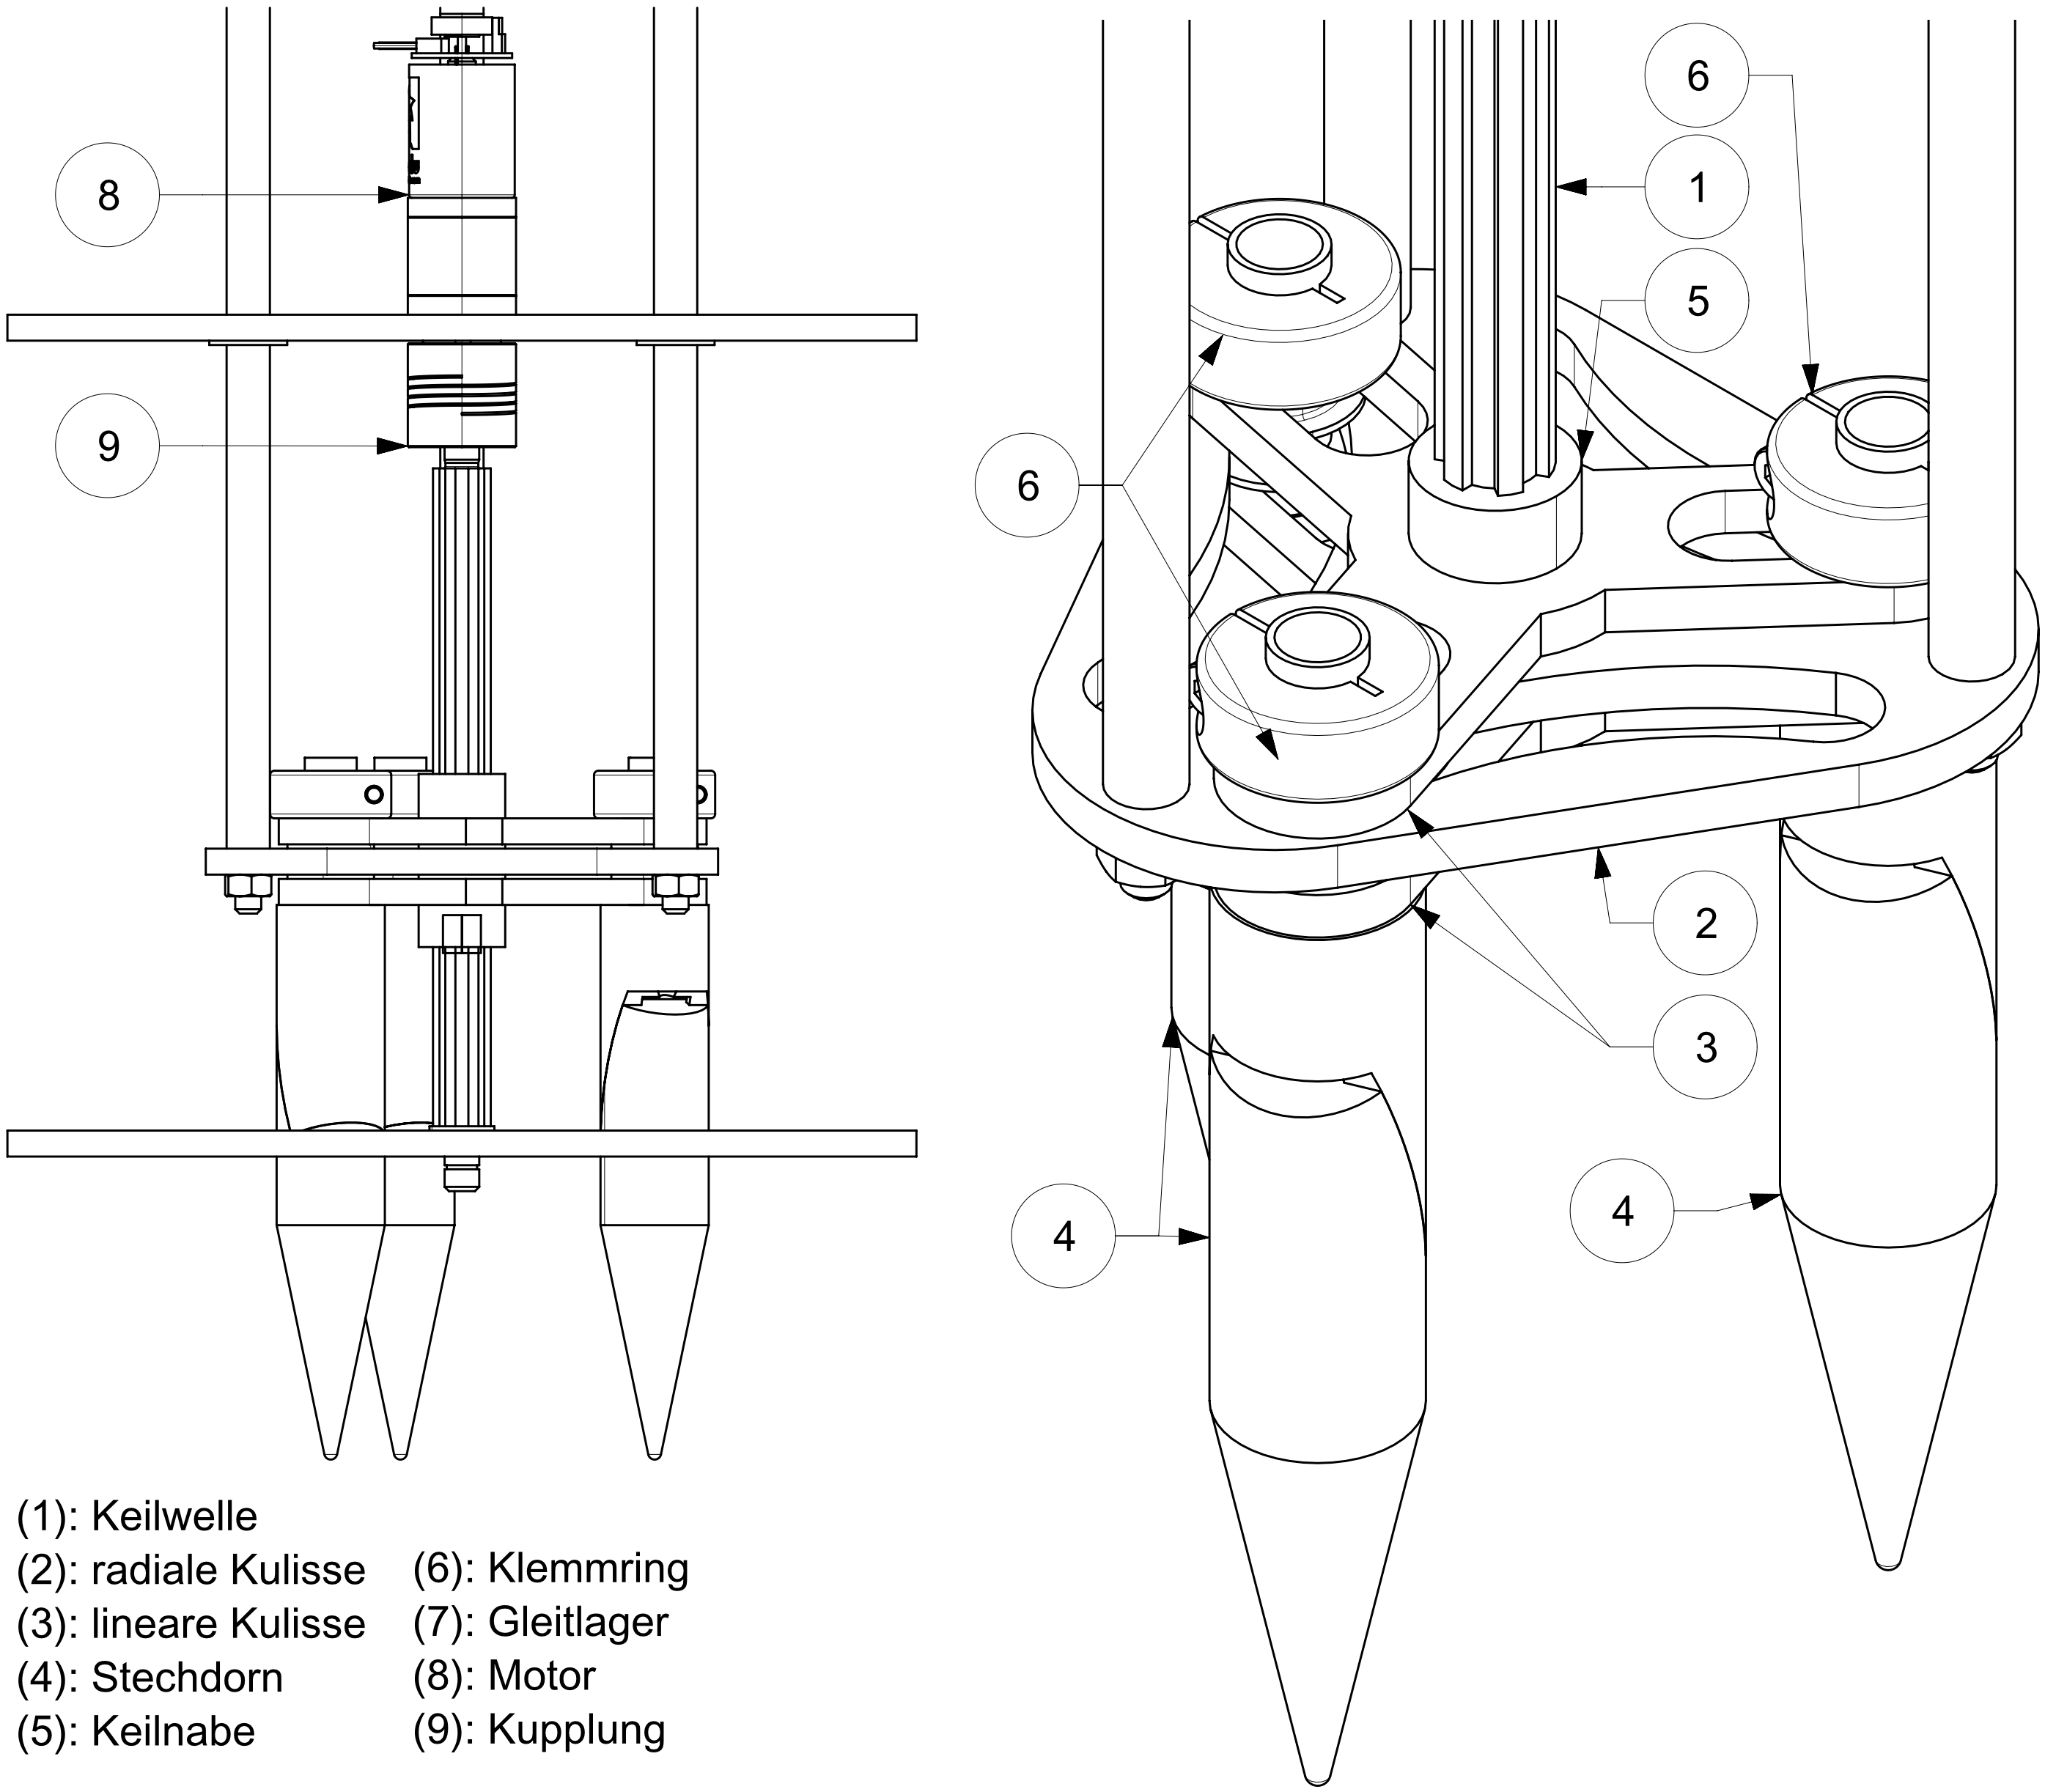
\includegraphics[scale=0.6]{Illustrationen/6-Umsetzung/details_vm.jpg}
	\caption{Detaillierte Übersicht der Verstellmechanik}
	\label{fig:details_vm}
	\end{figure}
Die Lagerung der Keilwelle wird nur wenig beansprucht, da durch die translatorische Freiheit der Keilnabe (entlang der Achse) keine Axialkräfte auftretten. Da die Verstellung des Topfradius nur wenige Male pro Tag vorgenommen wird, kann gemäss Roloff Matekk (Kapitel 14.3.1) von einer statischen Belastung (da n<10U/min) ausgegangen werden \cite{roloffmatek}. Daher ist die Verwendung eines Gleitlagers am unteren Ende (10) ausreichend. Verwendet wird das Gleitlager idlidur J3FM-0810 von Igus \cite{igusJ3FM}. Am oberen Ende ist die Keilwelle (1) über die Kupplung (9) durch den Getriebemotor (8) gelagert.
\newline

Der Stechdorn wird durch zwei lineare Kulissen (Punkt 3 in Abb \ref{fig:schnitt_vm}) und eine radiale Kulisse (2) geführt. Dabei sind die linearen Kulissen (3) mit der Keilnabe verbunden, die Radiale über die Führungen mit der Spindel. Um die Reibung zwischen Stechdorn und Kulissen zu vermindern werden auch hier Gleitlager (7) von igus eingesetzt. Die ganze Mechanik wird dabei durch die Auflage des Stechdorns (4) und einem Klemmring (6) gehalten.
	\begin{figure}[H]
	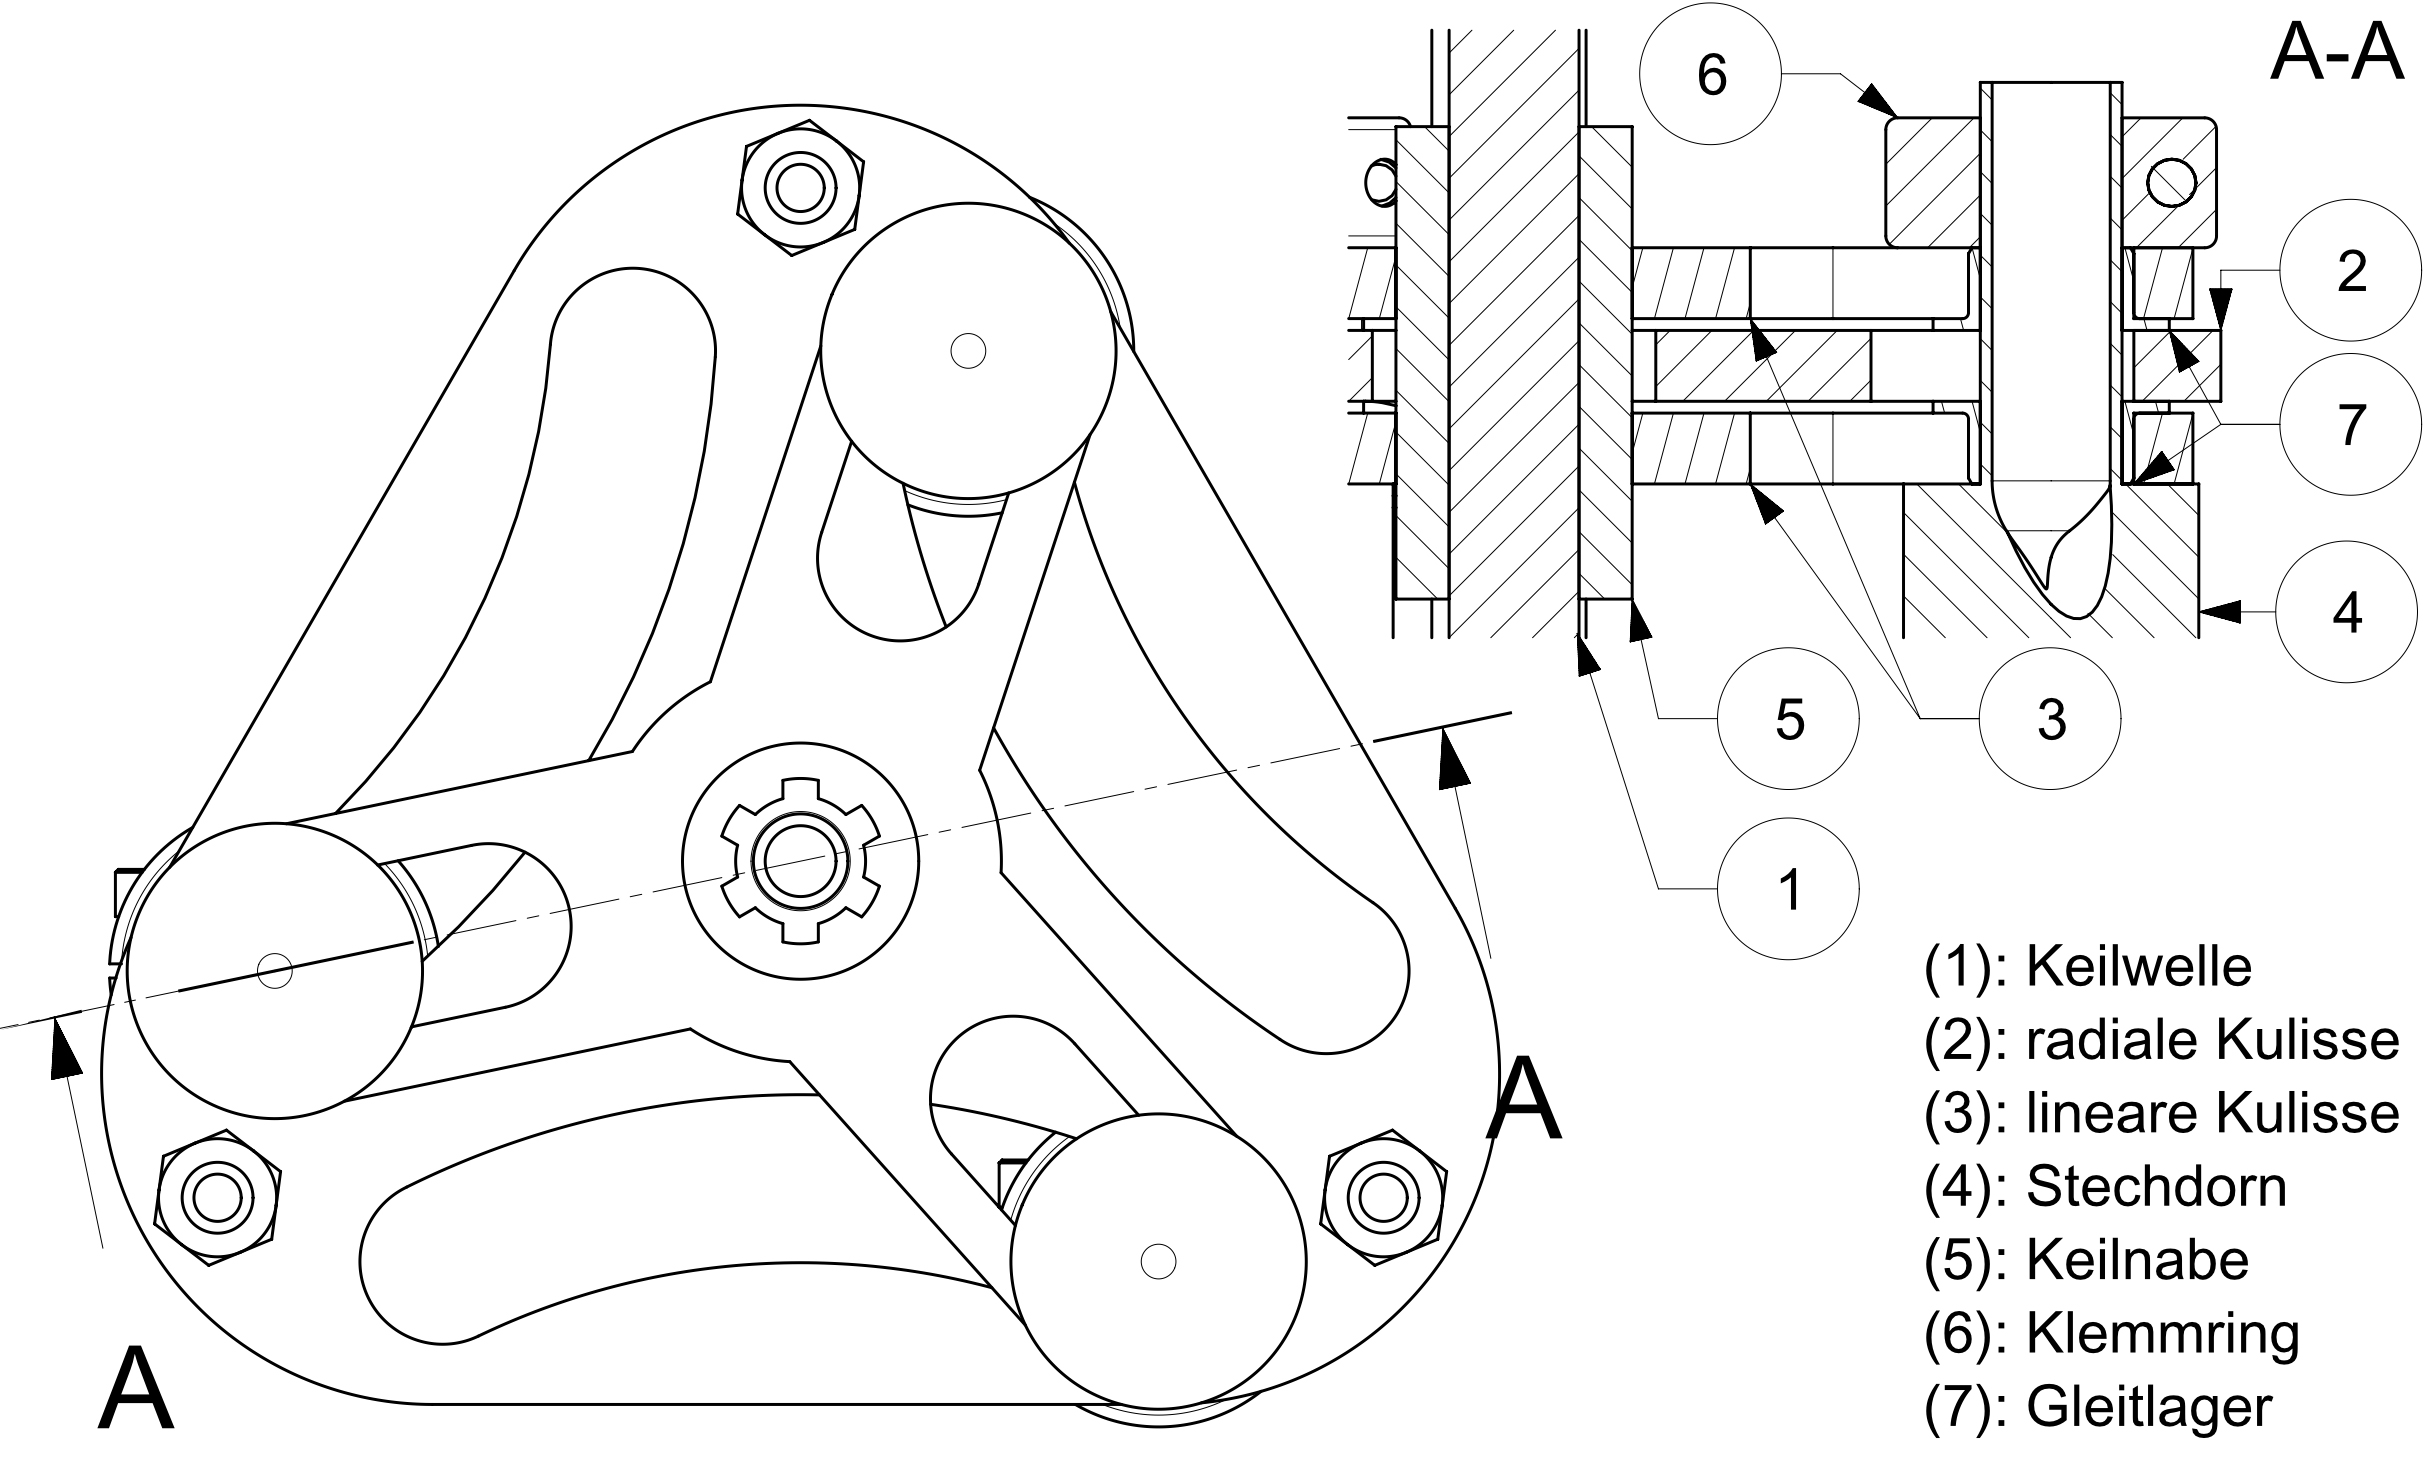
\includegraphics[scale=0.63]{Illustrationen/6-Umsetzung/schnitt_vm.jpg}
	\caption{Geschnittene Seitenansicht der Verstellmechanik}
	\label{fig:schnitt_vm}
	\end{figure}

\subsubsection{Funktion}
Die Bewegung der Verstellmechanik ist in Abbildung \ref{fig:motion_vm} dargestellt. Punkt B bildet ein beliebiger Punkt ab. Damit wird am Anschlag (Punkt A aus Abb. \ref{fig:motion_vm}) die Einsetzlokalität des grössten Topfes (Dmax = 140mm) und bei halbem Weg der Kulisse die Einsetzlokalität des kleinsten Topfes (Dmin = 90mm) erreicht. Dabei fällt auf, dass das Doppelte des nötigen Weges implementiert wurde. Begründet wird dies damit, dass dadurch der hochübersetzte Getriebemotor mehr Umdrehungen absolviert, bis der gewünschte Radius erreicht wird. Dies steigert die Auflösung des Motors und verbessert die Regelbarkeit.
	\begin{figure}[H]
	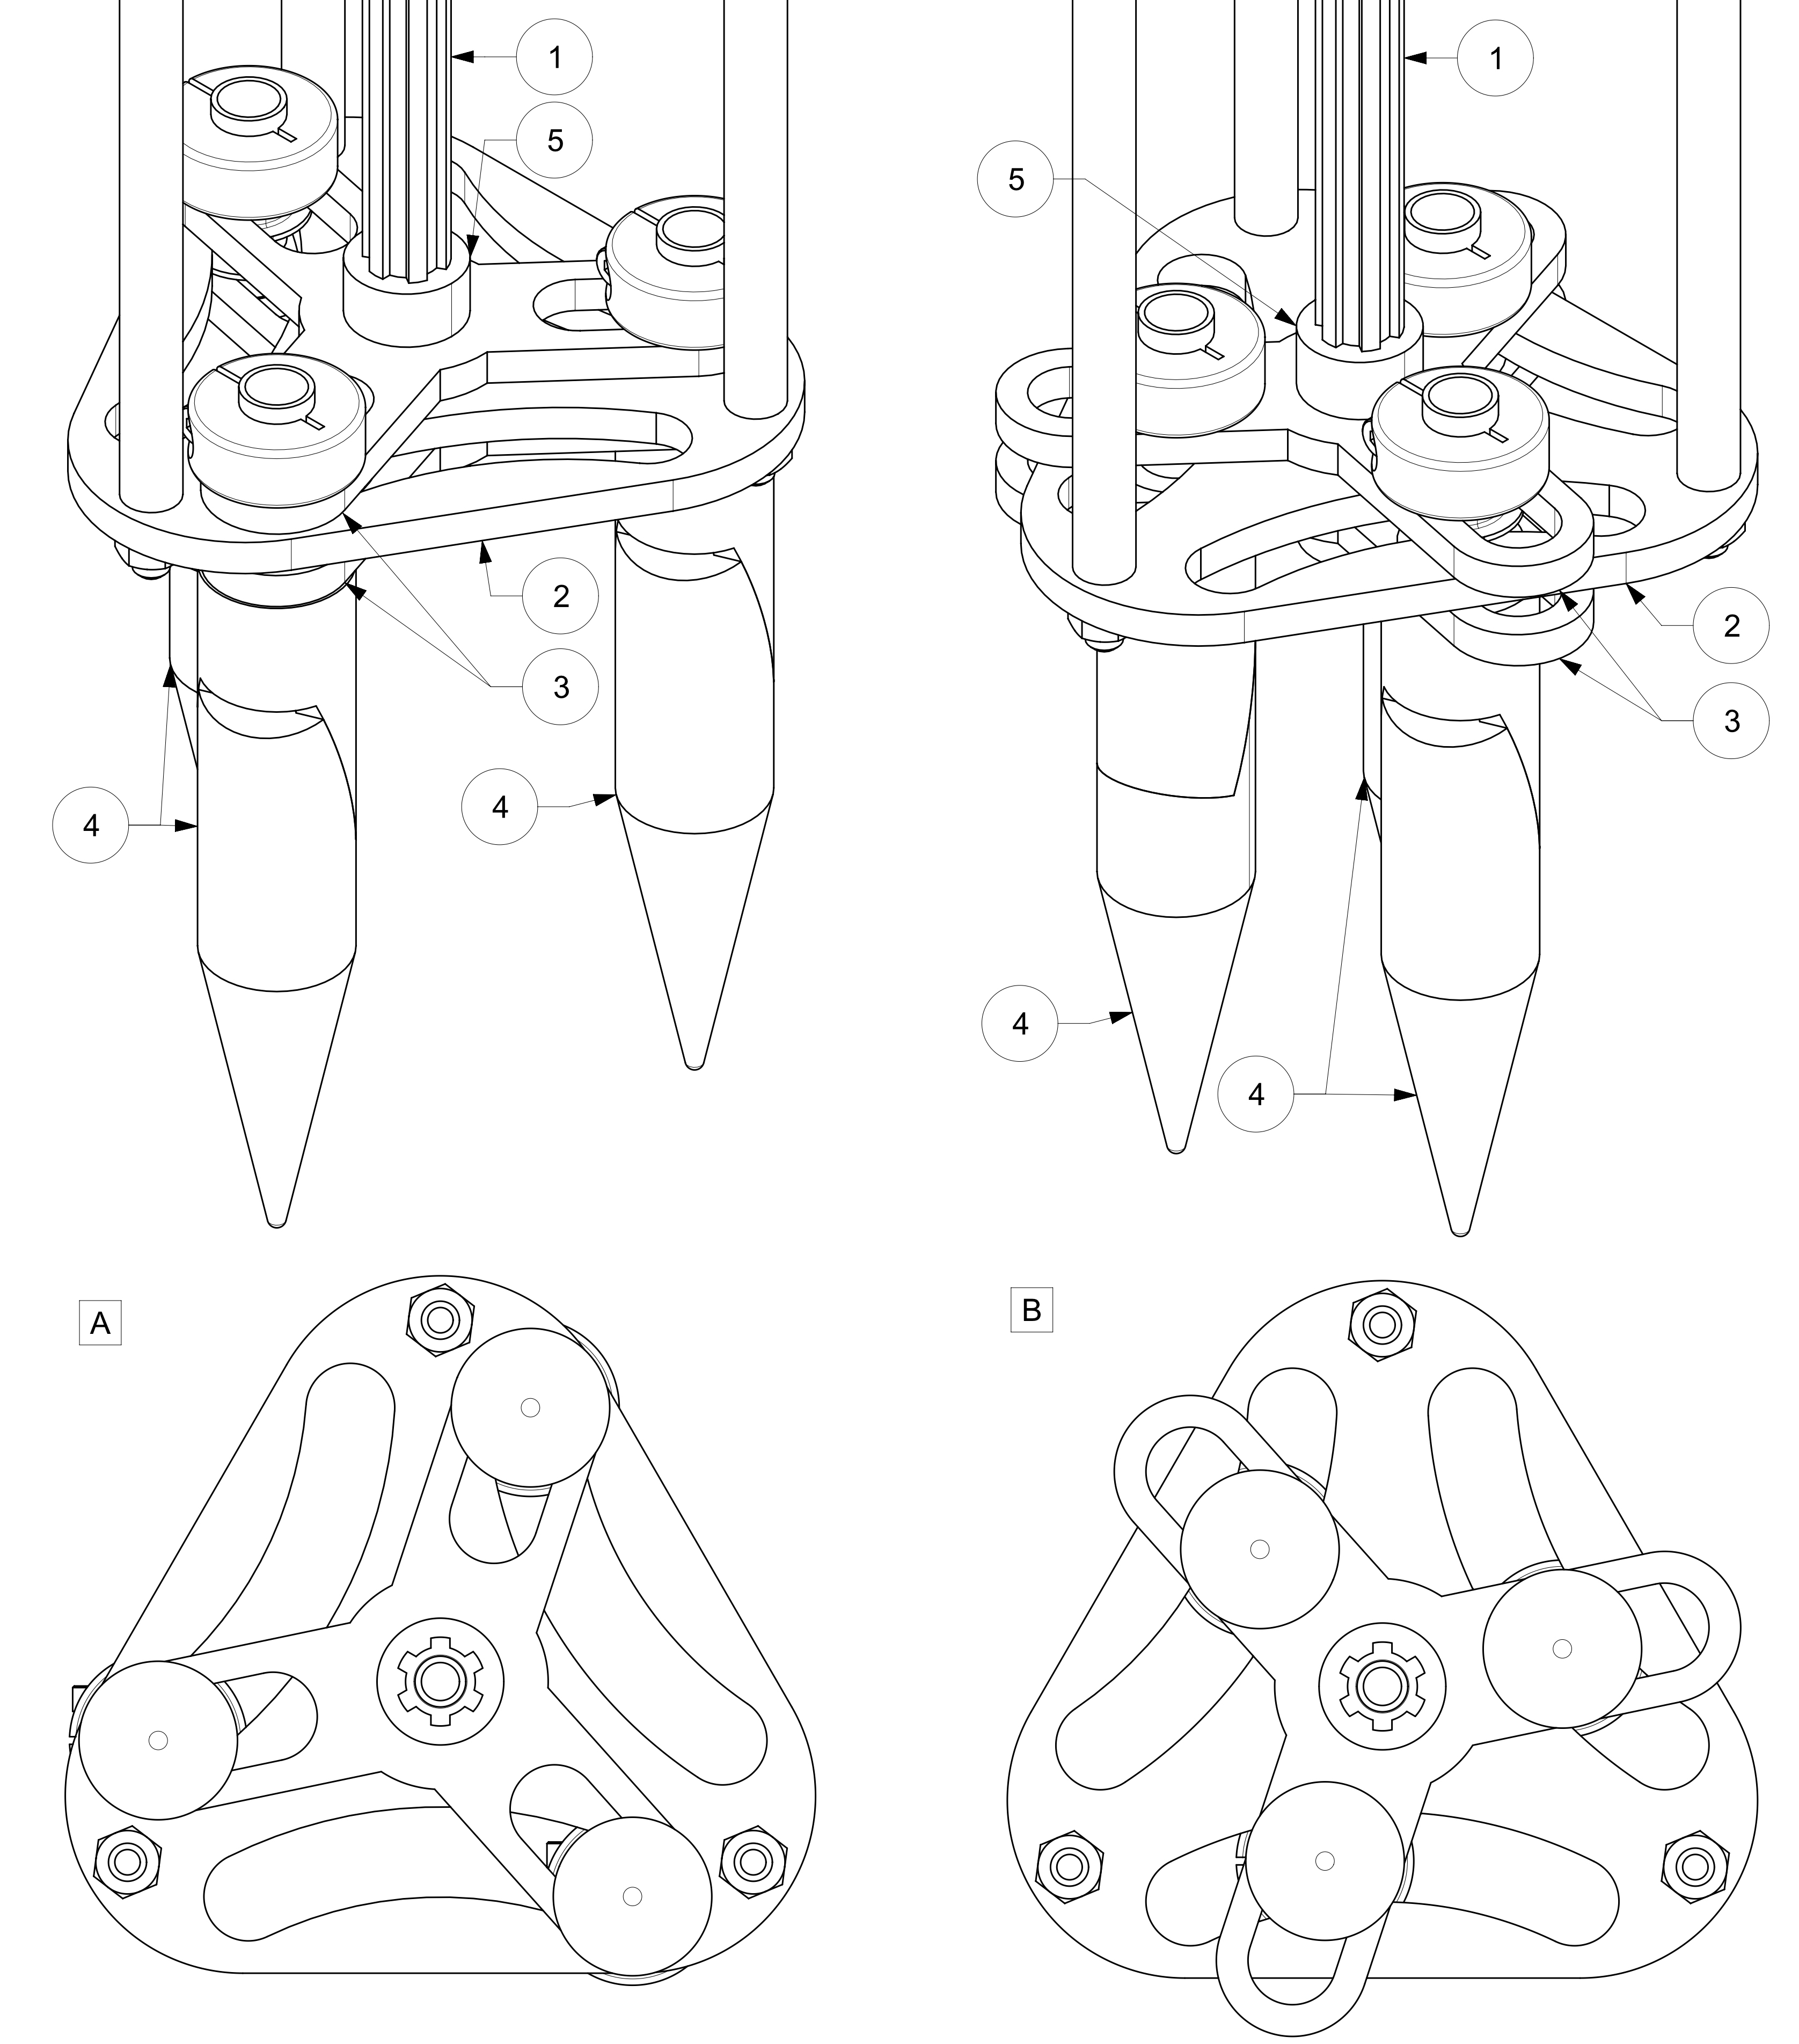
\includegraphics[scale=0.53]{Illustrationen/6-Umsetzung/motion_vm.jpg}
	\caption{Verstellung des Topfradius}
	\label{fig:motion_vm}
	\end{figure}

Wie schon erläutert, ist ein geringes Gewicht der beschleunigten Masse anzustreben. Gemäss Berechnungen soll die beschleunigte Masse maximal 1kg betragen. Um diese Anforderung zu erfüllen, werden die Kulissen (Punkte 2 und 3 aus Abb. \ref{fig:motion_vm}) aus 6mm dickem Aluminiumblech hergestellt.

\subsubsection{Prozessablauf}
\textit{(pro)} Genaue Spezifikationen für den Antrieb der Verstellmechanik zu definieren stellte sich als schwierig heraus. Da die einzigen Drehmomente, welche dem Antrieb entgegenwirken, auf Reibkräfte der Mechanik beruhen, welche schlecht geschätzt werden können. Eine weitere Herausforderung bergen die kleinen Winkeländerungen an der Antriebswelle des Motors (der ganze Bewegungsraum von Anschlag zu Anschlag beträgt ca. 100°). Um solch kleine Winkeländerungen präzise fahren zu können wird ein DC Getriebemotor von Pololu mit einer Getriebeübersetzung von 378:1 verwendet.  Die Spezifikationen, sowie die Begründung für die Wahl dieser Antriebstechnik sind in Kapitel \ref{kap:Evaluation_der_Komponenten} erläutert.\\
Der Prozessablauf zur Initialisierung sowie das Einstellen verschiedener Topfgrössen ist in Abb. \ref{fig:Prozessablauf_Verstellmechanik} illustriert. Wie bei der Setzeinheit wird die Verstellmechanik durch das Anfahren eines mechanischen Anschlags initialisiert. Die verschiedenen Topfgrössen von 9cm... 14cm können durch fahren einer relativen Schrittweite zum Anschlag eingestellt werden.

\begin{figure}[H]
	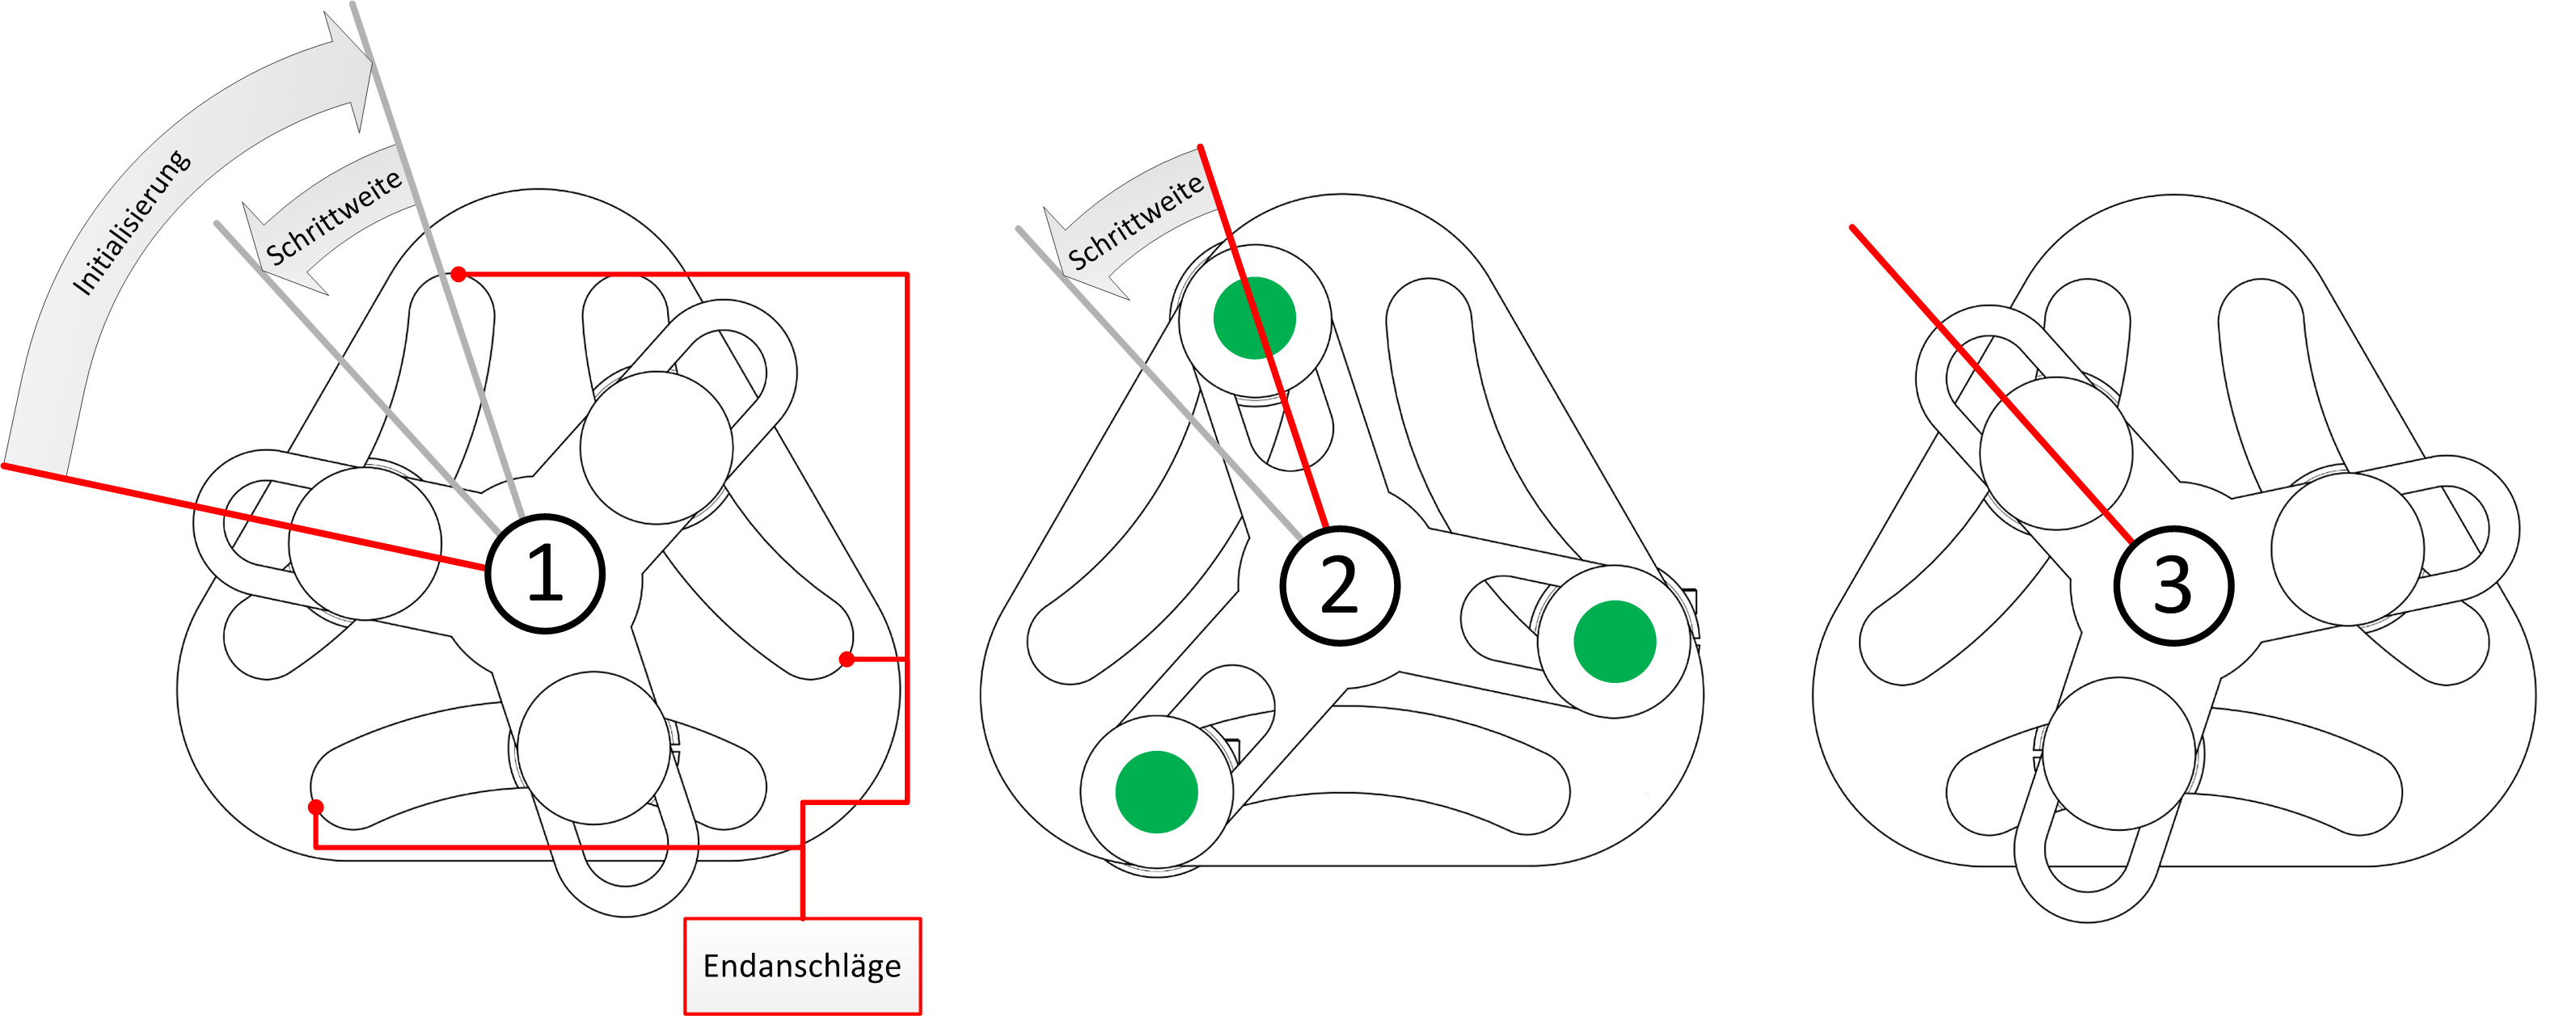
\includegraphics[width=1\textwidth]{Illustrationen/6-Umsetzung/Prozessablauf_Verstellmechanik.png}
	\caption{Prozessablauf der Verstellmechanik}
	\label{fig:Prozessablauf_Verstellmechanik}
\end{figure}

Der Prozess wurde in drei Etappen unterteilt welche mit den Ziffern 1... 3 nummeriert sind. Im folgenden Abschnitt werden die drei Etappen erläutert:

\begin{enumerate}
	\item Nach einem Neustart der Maschine befindet sich die Verstellmechanik in einer unbekannten Position. Um die absolute Position der Verstellmechanik zu ermitteln wird diese an die mechanischen Endanschläge der Führungskullise bewegt. Durch die Erhöhung des Laststroms wird der Endanschlag vom uC erkannt.
	\item In dieser Etappe befindet sich die Verstellmechanik an den Endanschläge. Dies wurde durch grüne Kreise, an den jeweiligen Punkten wo die Mechanik den Endanschlag berührt, gekennzeichnet.
	\item Durch bewegen der Verstellmechanik um eine definierte Schrittweite relativ zum Endanschlag können nun die verschiedenen Setzradien eingestellt werden. Aufgrund der Form der Führungskulisse ergeben sich jeweils zwei Positionen, links und rechts vom kleinsten Setzradius, für die Topfgrössen 11cm, 12cm, 13cm und 14cm.
\end{enumerate}

Die Parameter für die Schrittweiten der jeweiligen Setzradien werden im Kapitel Inbetriebnahme (\ref{sec:Inbetriebnahme_Verstellmechanik}) behandelt.